\documentclass[12pt]{article}
\usepackage{amsmath}
\usepackage{graphicx}
\usepackage{hyperref}
\usepackage[utf8]{inputenc}
\usepackage[spanish]{babel}
\usepackage[margin=3cm]{geometry}
\usepackage{amsfonts}
\usepackage{listings}
\usepackage[T1]{fontenc}
\usepackage{float}
\usepackage{subfig}

\title{Practica 4 - Visión por Computador.}
\author{Néstor Rodríguez Vico. DNI: 75573052C - \href{mailto:nrv23@correo.ugr.es}{nrv23@correo.ugr.es}}
\date{\today}


\lstdefinestyle{bash_style}{
	language=bash,
	frame=single,
	xleftmargin=.25in,
	upquote = true,
	basicstyle=\scriptsize,
	breakatwhitespace=false,         
	breaklines=true,                 
	captionpos=b,                    
	keepspaces=true,                 
	numbers=left,                    
	numbersep=5pt,                  
	showspaces=false,                
	showstringspaces=false,
	showtabs=false,                  
	tabsize=2
}

\lstset{style=bash_style}

\begin{document}
\maketitle

\setlength{\belowdisplayskip}{5pt} 
\setlength{\belowdisplayshortskip}{5pt}
\setlength{\abovedisplayskip}{5pt} 
\setlength{\abovedisplayshortskip}{5pt}

\section{Moravec.}

A continuación se muestra el resultado del algoritmo de Moravec. La idea aplicada está en los comentarios del código.

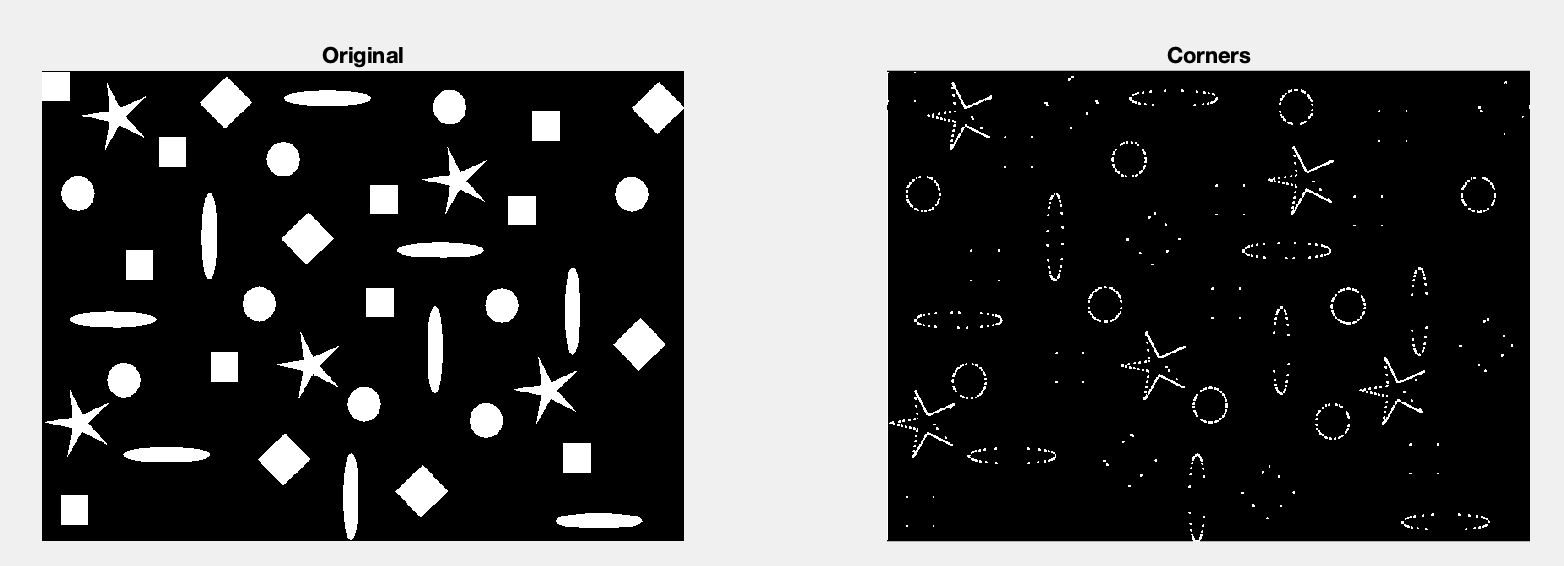
\includegraphics[width=\linewidth]{images/moravec.png}

\section{Ejercicio 3.}

Los resultados del ejercicio tres (buscar patrones) son los siguientes:

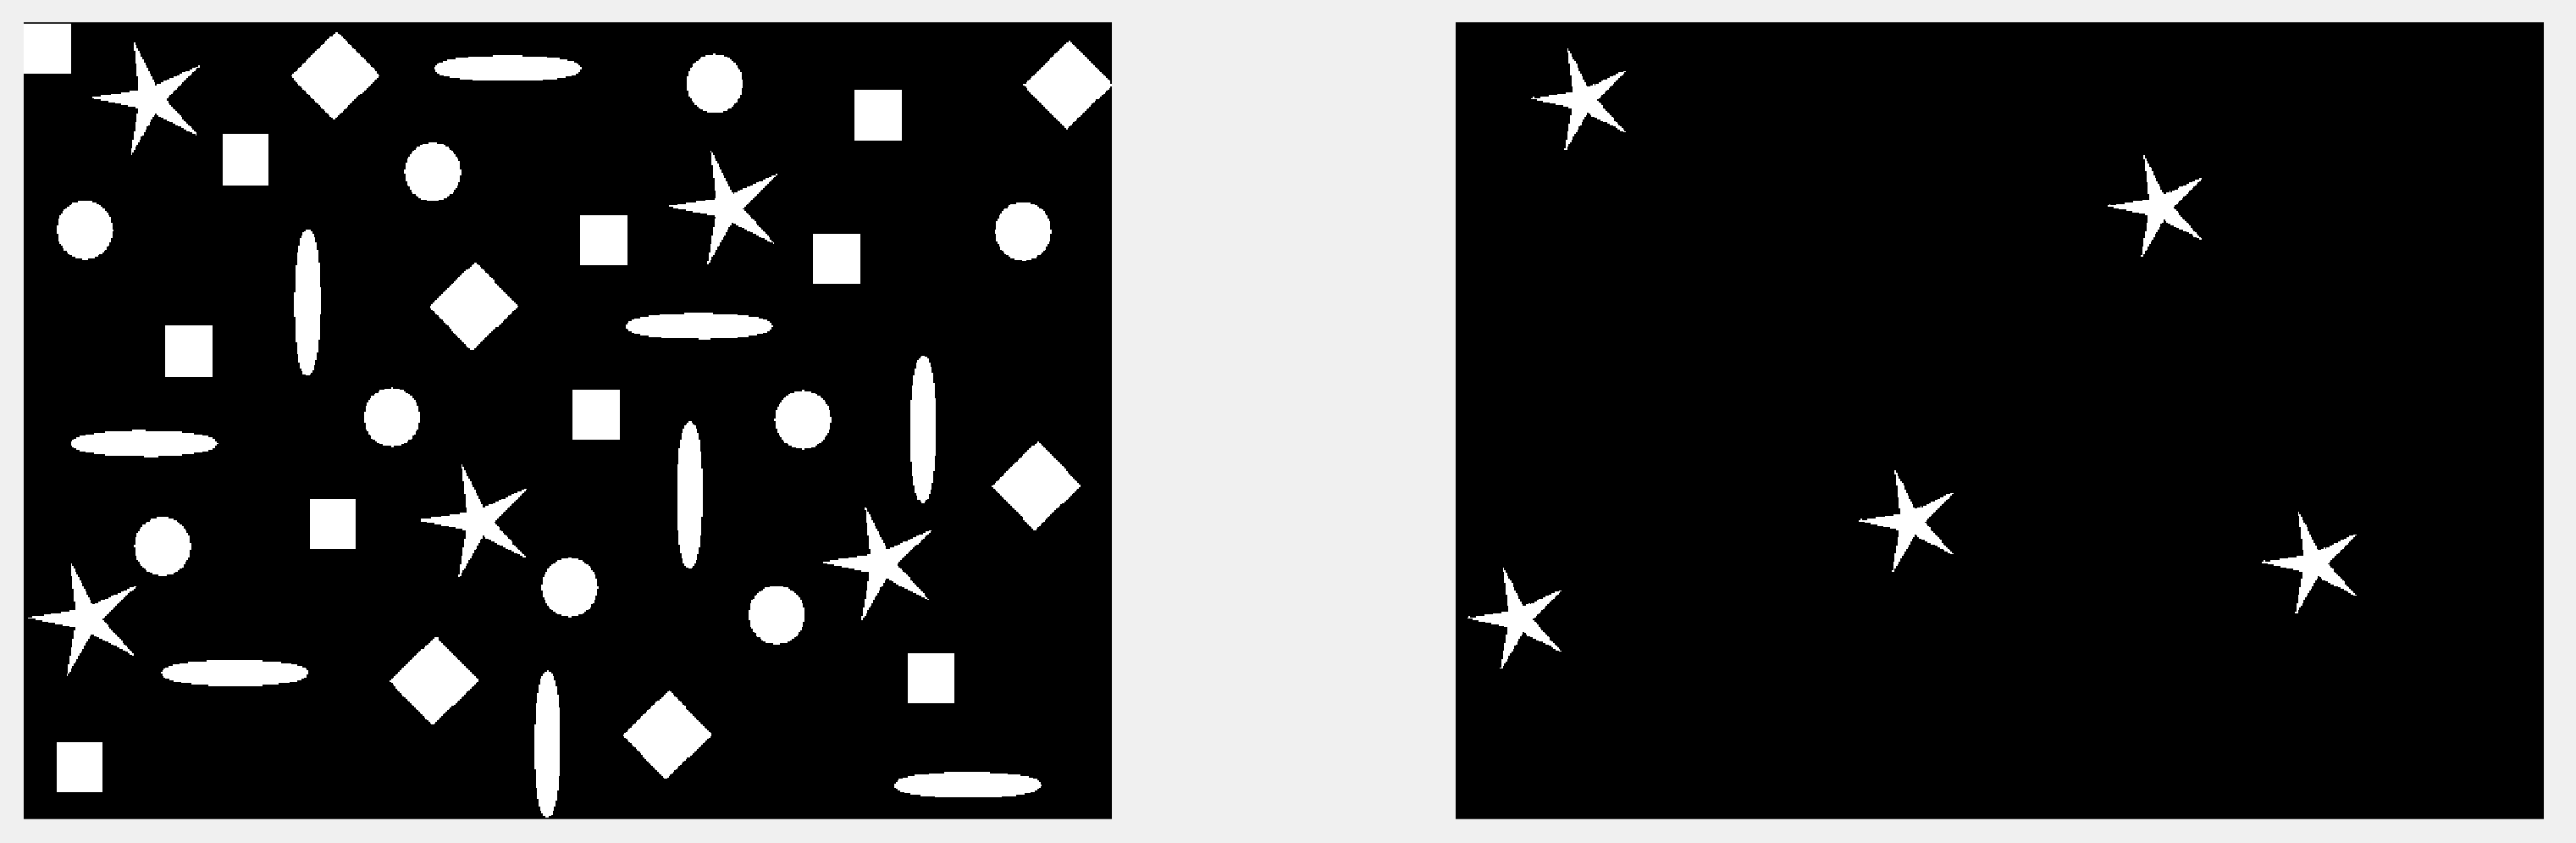
\includegraphics[width=\linewidth]{images/figuras.png}

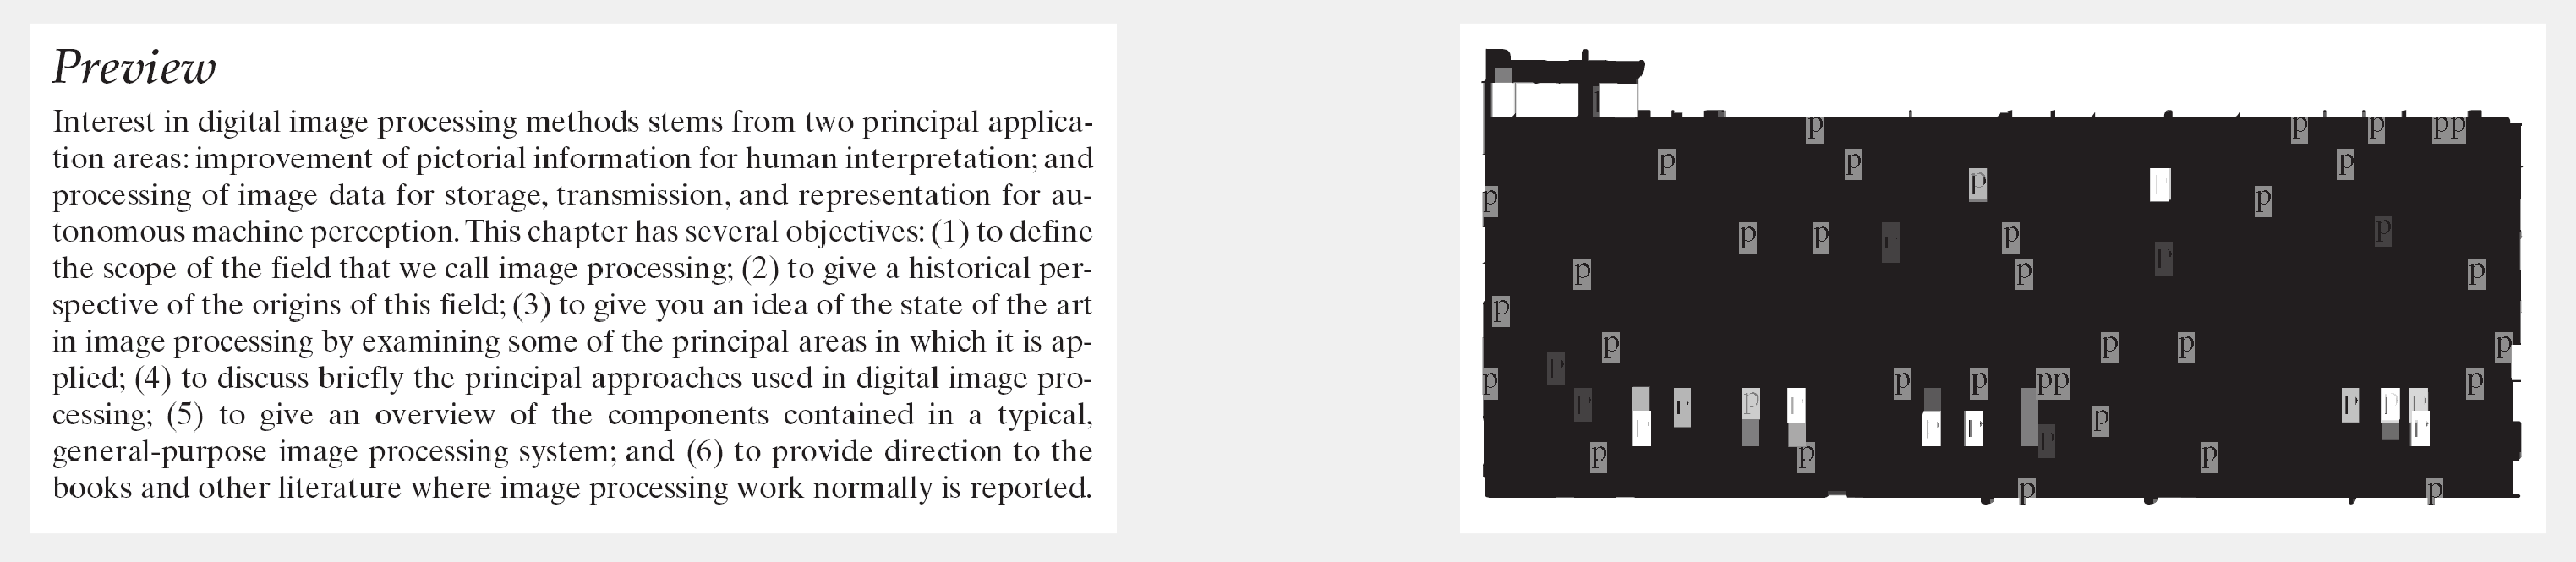
\includegraphics[width=\linewidth]{images/letra_p.png}

El resultado de mi idea documentada en el código es el siguiente:

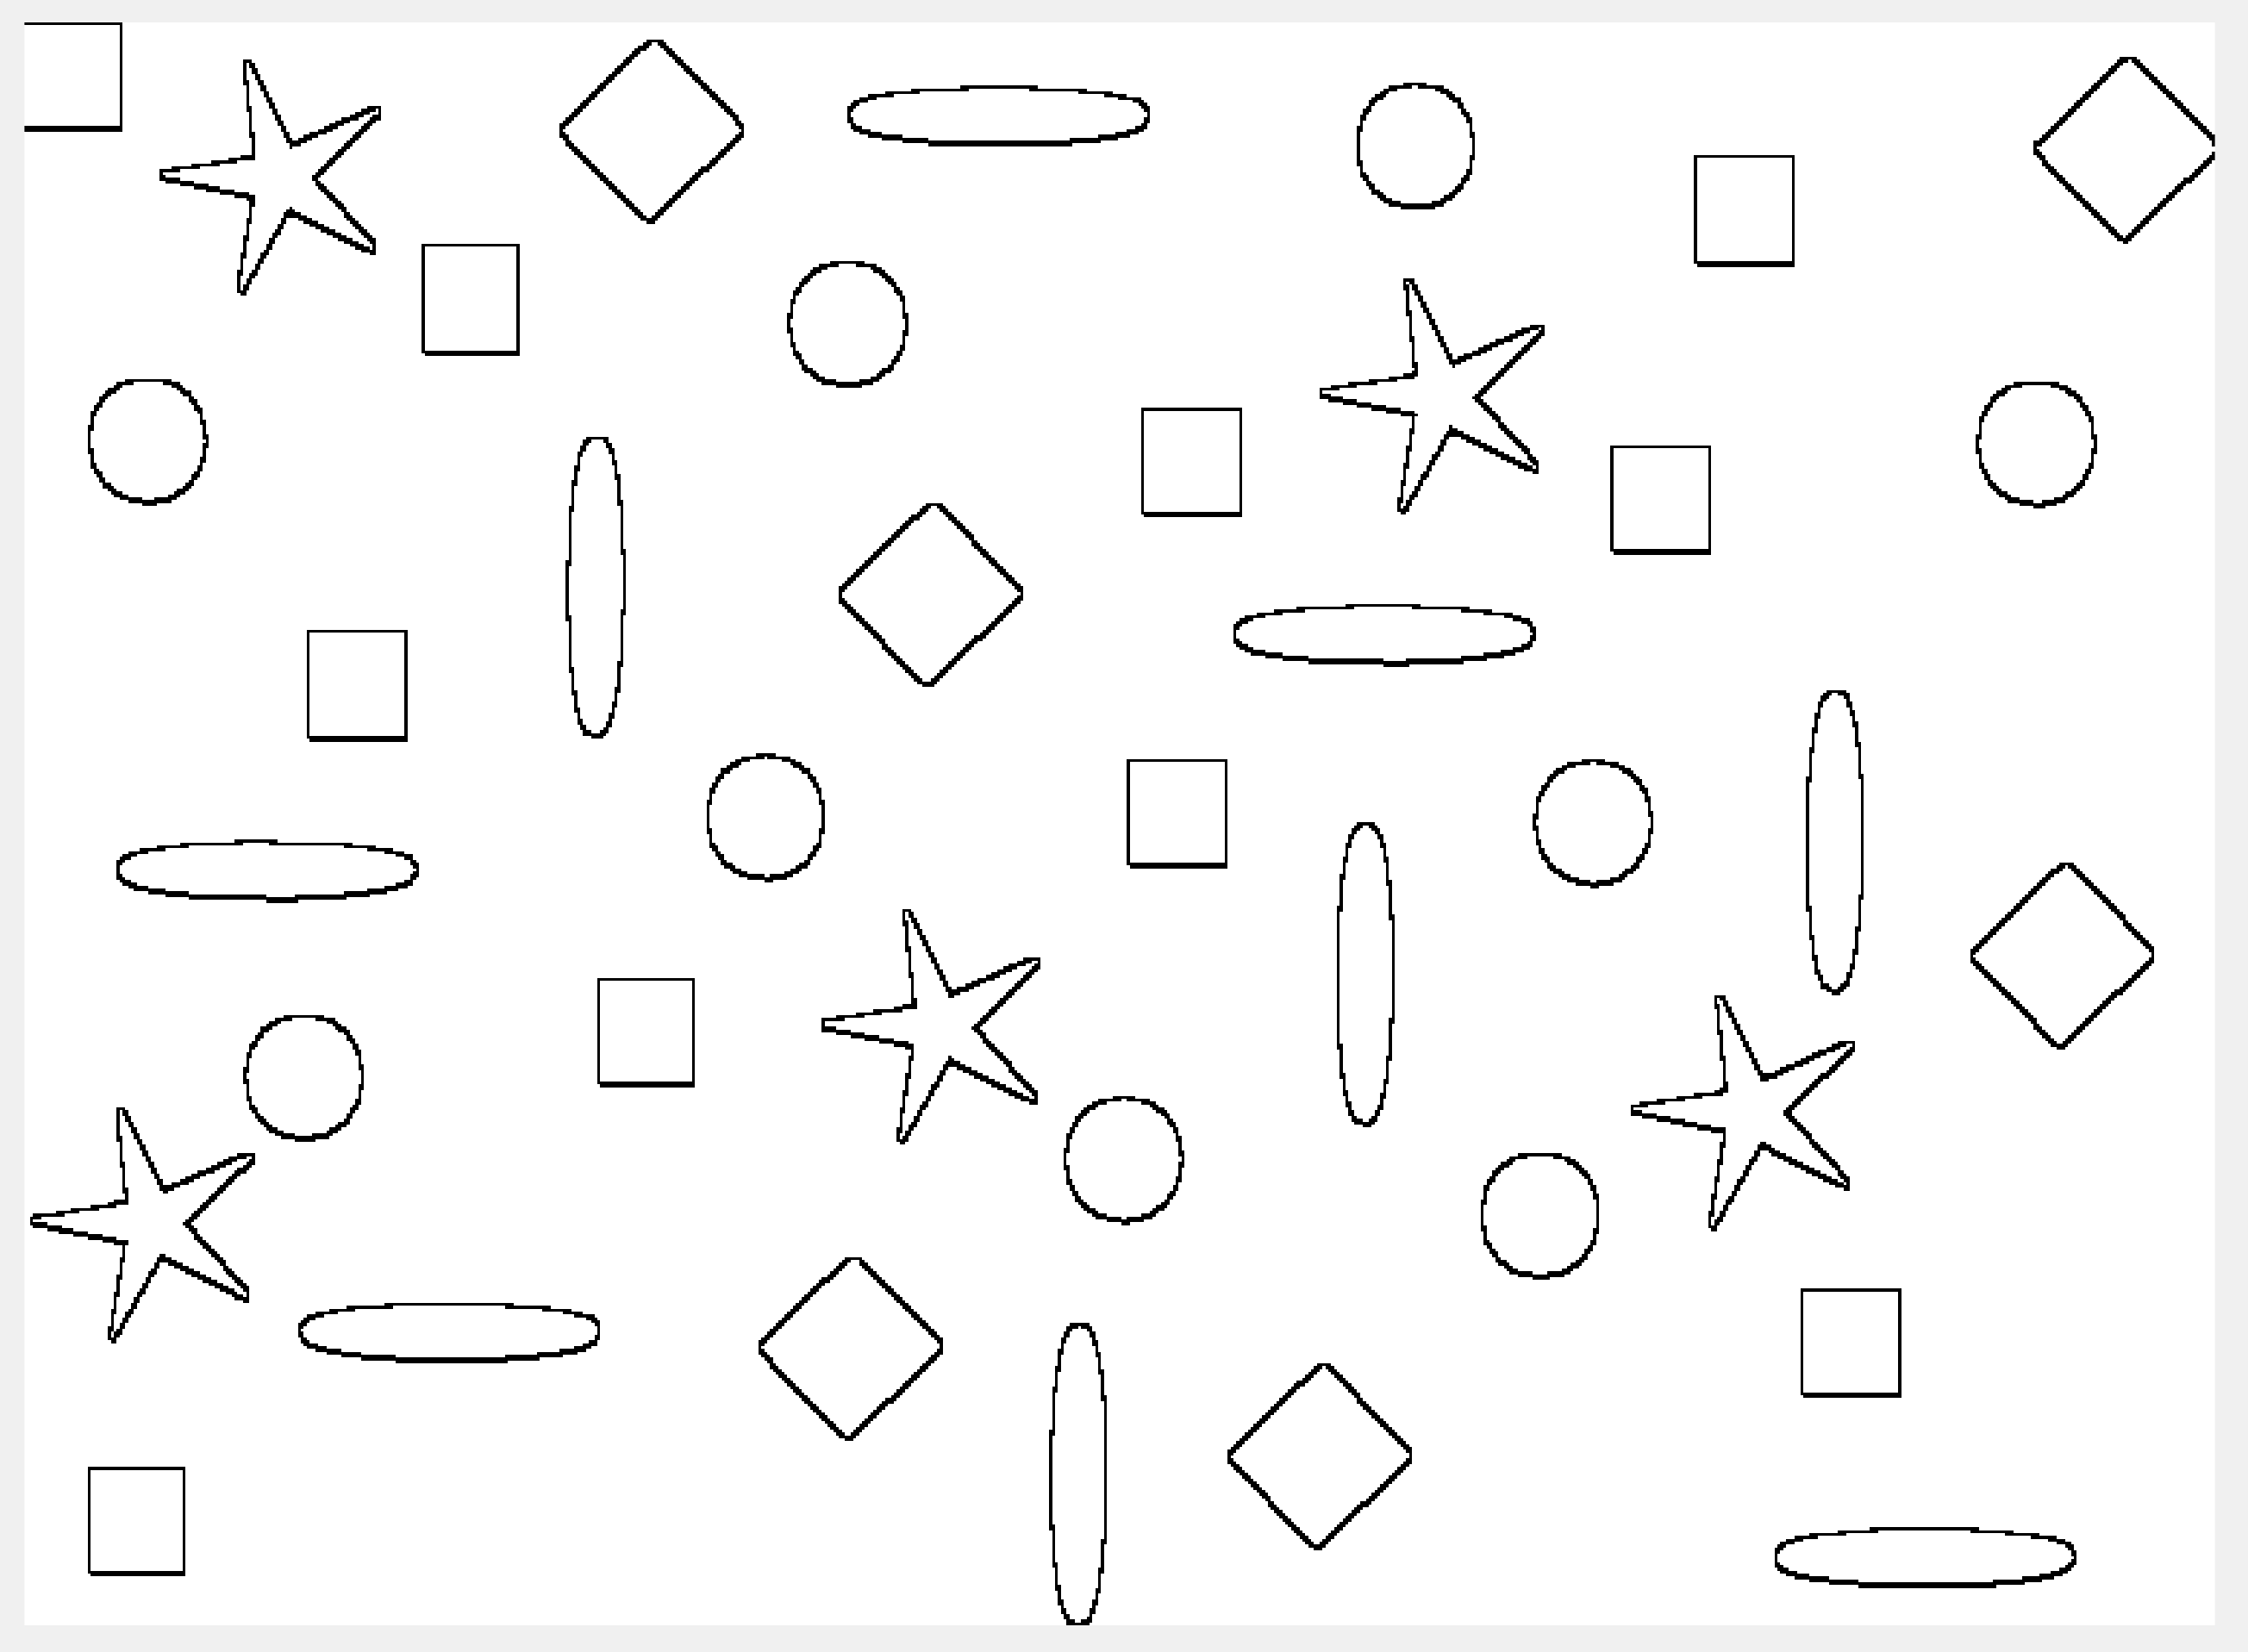
\includegraphics[width=\linewidth]{images/figuras_custom.png}

He intentado aplicar dicha idea para las letras pero no he obtnido un buen resultado debido al tamaño de los patrones a buscar...

\end{document}